\documentclass[12pt]{article}
\usepackage[utf8]{inputenc}

\usepackage{enumitem}
\usepackage[margin=2cm]{geometry}

\usepackage{amsmath, amsfonts, amssymb}
\usepackage{graphicx}
\usepackage{tikz}
\usepackage{pgfplots}
\usepackage{multicol}

\usepackage{comment}
\usepackage{url}
\usepackage{calc}
\usepackage{subcaption}

\usepackage{array}

\usepackage{fancyhdr}
\pagestyle{fancy}
\fancyhf{}
\renewcommand{\headrulewidth}{2pt}
\renewcommand{\footrulewidth}{0pt}
\rfoot{\thepage}
\lhead{\textsc{Math} 244}
\chead{\textsc{Homework 1}}
\rhead{Fall 2023}

\pgfplotsset{compat=1.16}

% MATH commands
\newcommand{\ga}{\left\langle}
\newcommand{\da}{\right\rangle}
\newcommand{\oa}{\left\lbrace}
\newcommand{\fa}{\right\rbrace}
\newcommand{\oc}{\left[}
\newcommand{\fc}{\right]}
\newcommand{\op}{\left(}
\newcommand{\fp}{\right)}

\newcommand{\bi}{\mathbf{i}}
\newcommand{\bj}{\mathbf{j}}
\newcommand{\bk}{\mathbf{k}}
\newcommand{\bF}{\mathbf{F}}

\newcommand{\ra}{\rightarrow}
\newcommand{\Ra}{\Rightarrow}

\newcommand{\sech}{\mathrm{sech}\,}
\newcommand{\csch}{\mathrm{csch}\,}
\newcommand{\curl}{\mathrm{curl}\,}
\newcommand{\dive}{\mathrm{div}\,}

\newcommand{\ve}{\varepsilon}
\newcommand{\spc}{\vspace*{0.5cm}}

\DeclareMathOperator{\Ran}{Ran}
\DeclareMathOperator{\Dom}{Dom}

\newcommand{\exo}[3]{\noindent\textcolor{red}{\fbox{\textbf{Section {#1}, Problem {#2}}}\hrulefill   \textbf{({#3} Pts})}\\}

\begin{document}
\thispagestyle{empty}
	\noindent \hrulefill \\
	MATH-244 \hfill Pierre-Olivier Paris{\'e}\\
	Homework 1 Solutions \hfill Fall 2023\\\vspace*{-0.7cm}
	
	\noindent\hrulefill
	
	\spc
	
	\exo{15.1}{4a}{10}
	\\
	We have $\Delta x = (2 - 1)/2 = 0.5$ and $\Delta y = (3 - 0)/2 = 1.5$. The rectangle is then divided in the way shown in the figure below:
		\begin{center}
		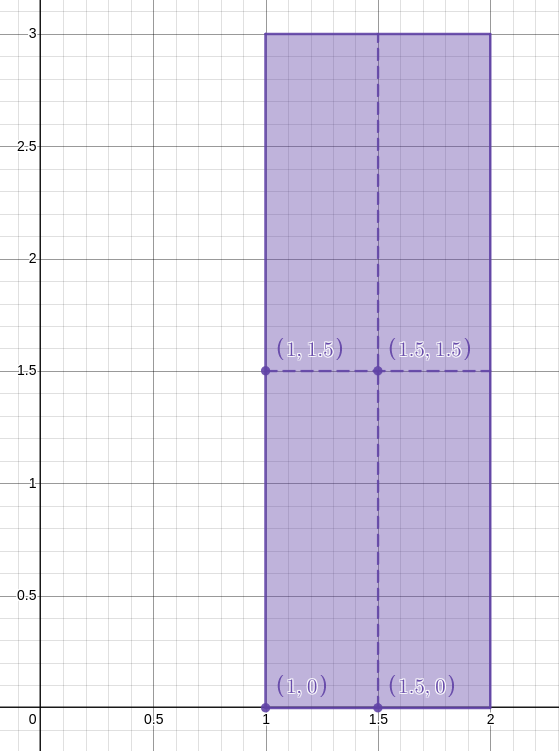
\includegraphics[scale=0.5]{rectangle.png}
		\end{center}
	In the above picture, the coordinates of the bottom left corners of each sub-rectangle are $(x_{11}^\ast , y_{11}^\ast) = (1, 0)$, $(x_{12}^\ast , x_{12}^\ast) = (1, 1.5)$, $(x_{21}^\ast , y_{21}^\ast ) = (1.5, 0)$, and $(x_{22}^\ast , y_{22}^\ast) = (1.5, 1.5)$. The Area of each sub-rectangle is $0.5 \cdot 1.5 = 0.75$. We first have
		\begin{align*}
		(1 + 1^2 + (3)(0)) + (1 + 1^2 + (3) (1.5)) + (1 + 1.5^2 + (3)(0)) + (1 + 1.5^2 + (3) (1.5)) = 19.5 ,
		\end{align*}
	and then
		\begin{align*}
		V \approx 19.5 \cdot 0.75 = 14.625 .
		\end{align*} .

	\newpage

	\exo{15.1}{16}{10}
	\\
	Setting $u = x + y$, 
		\begin{align*}
		\int_0^1 (x + y)^2 \, dx = \int_y^{1 + y} u^2 \, du = \frac{(1 + y)^3}{3} - \frac{y^3}{3} .
		\end{align*}
	Then, 
		\begin{align*}
		\int_0^1 \int_0^1 (x + y)^2 \, dx dy &= \int_0^1 \Big( \frac{(1 + y)^3}{3} - \frac{y^3}{3} \Big) \, dy \\
		&= \int_0^1 \frac{(1 + y)^3}{3} \, dy - \int_0^1 \frac{y^3}{3} \, dy .
		\end{align*}
	Setting $v = 1 + y$, 
		\begin{align*}
		\int_0^1 \frac{(1 + y)^3}{3} \, dy &= \int_1^2 \frac{v^3}{3} \, dv \\
		&= \frac{2^4}{12} - \frac{1}{12} = \frac{15}{12} .
		\end{align*}
	Also,
		\begin{align*}
		\int_0^1 \frac{y^3}{3} \, dy = \frac{1}{12} - 0 = \frac{1}{12} .
		\end{align*}
	So,
		\begin{align*}
		\int_0^1 \int_0^1 (x + y)^3 \, dx dy = \frac{15}{12} - \frac{1}{12} = \frac{7}{6} \approx 1.1667 . \tag*{$\triangle$}
		\end{align*}

	\spc 

	\exo{15.1}{20}{10}
	\\
	With $u = \ln y$, we have $du = \frac{dy}{y}$ and so
		\begin{align*}
		\int_1^5 \frac{\ln y}{xy} \, dy = \int_0^{\ln 5} \frac{u}{x} \, du = \frac{(\ln 5)^2}{2x} .
		\end{align*}
	Then,
		\begin{align*}
		\int_1^3 \int_1^5 \frac{\ln y}{xy} \, dy dx &= \int_1^3 \frac{(\ln 5)^2}{2x} \, dx \\
		&= \frac{(\ln 5)^2}{2} (\ln 3 - \ln 1)\\
		& = \frac{(\ln 5)^2 (\ln 3)}{2} \approx 1.4228 . \tag*{$\triangle$}
		\end{align*}

	\spc 

	\exo{15.1}{22}{10}
	\\
	Using the fact that $e^{x - y} = e^xe^{-y}$,
		\begin{align*}
		\int_0^1 \int_0^2 y e^{x - y} \, dx dy &= \int_0^1 \int_0^2 e^x y e^{-y} \, dx dy \\
		&= \Big( \int_0^2 e^x \, dx \Big) \Big( \int_0^1 ye^{-y} \, dy \Big) .
		\end{align*}
	We compute
		\begin{align*}
		\int_0^2 e^x \, dx = e^2 - 1 .
		\end{align*}
	Then, from an integration by parts, 
		\begin{align*}
		\int_0^1 y e^{-y} \, dy &= \left. (-ye^{-y}) \right|_0^1 + \int_0^1 e^{-y} \, dy \\
		&= -e^{-1} + (1 - e^{-1}) .
		\end{align*}
	Therefore,
		\begin{align*}
		\int_0^1 \int_0^2 y e^{x -y} \, dx dy &= (e^2 - 1) (-e^{-1} + 1 - e^{-1}) \\
		&= -e + e^{-1} + e^2 - 1 - e + e^{-1} \\
		&= -1 + 2e^{-1} + (e - 2) e \\
		& \approx 1.6883 . \tag*{$\triangle$}
		\end{align*}

	\spc 

	\exo{15.1}{34}{10}
	\\
	Using Fubini's Theorem, 
		\begin{align*}
		\iint_R \frac{1}{1 + x + y} \, dA = \int_{1}^2 \int_1^3 \frac{1}{1 + x + y} \, dx dy .
		\end{align*}
	Letting $u = 1 + x + y$, we have $du = dx$, so that
		\begin{align*}
		\int_1^3 \frac{1}{1 + x + y} \, dx &= \int_{2 + y}^{4 + y} \frac{1}{u} \, du \\
		&= \ln (4 + y) - \ln (2 + y) .
		\end{align*}
	Then,
		\begin{align*}
		\int_1^2 \int_1^3 \frac{1}{1 + x +y} \, dx dy &= \int_1^2 \ln (4 + y) - \ln (2 + y) \, dy \\
		&= \int_1^2 \ln (4 + y) \, dy - \int_1^2 \ln (2 + y) \, dy .
		\end{align*}
	From an integration by part with $u = \ln (4 + y)$ and $dv = dx$, we obtain
		\begin{align*}
		\int_1^2 \ln (4 + y) \, dy &= \left. \Big[ (4 + y) \ln (4 + y) - y \Big] \right|_1^2 \\
		&= 6 \ln (6) - 5 \ln (5) - 1
		\end{align*}
	and similarly, we obtain
		\begin{align*}
		\int_1^2 \ln (2 + y) \, dy = 4 \ln (4) - 3 \ln (3) - 1 .
		\end{align*} 
	Therefore, 
	\begin{align*}
	\int_1^2 \int_1^3 \frac{1}{1 + x + y} \, dx dy&= 6 \ln (6) - 5 \ln (5) - 1 - 4 \ln (4) + 3 \ln (3) + 1 \\
	&= 9 \ln (3) - 2 \ln (2) - 5 \ln (5) \\
	& \approx 0.4540 . \tag*{$\triangle$}
		\end{align*}	

\vfill

\hfill \textsc{Total:} 50 Pts.

\end{document}